\documentclass[10pt]{article}
\usepackage[margin=0.78in]{geometry}
\usepackage[T1]{fontenc}
\usepackage{lmodern,microtype,amsmath,amssymb,booktabs,array,longtable,graphicx,xcolor,tikz,listings,enumitem}
\usetikzlibrary{arrows.meta,positioning,calc,fit}
\usepackage[colorlinks=true,allcolors=blue!45!black]{hyperref}
\hypersetup{pdftitle={Learning Reusable Safety Memory for VLA Policies},pdfauthor={Research design proposal}}
\definecolor{ink}{RGB}{35,64,87}
\definecolor{mem}{RGB}{29,110,86}
\definecolor{learn}{RGB}{160,87,35}
\setlength{\parindent}{0pt}
\setlength{\parskip}{5pt}
\setlength{\emergencystretch}{3em}
\setlist{nosep,leftmargin=*}
\lstset{basicstyle=\ttfamily\small,breaklines=true,columns=fullflexible,frame=single,rulecolor=\color{black!20}}
\newcommand{\code}[1]{\texttt{\detokenize{#1}}}
\title{Learning Reusable Safety Memory for VLA Policies\\\large A minimal design, its failure modes, and a PSC experiment plan}
\author{Research design proposal}
\date{11 October 2026}
\begin{document}
\maketitle
\vspace{-1.5em}
\begin{abstract}
Keep the existing VLA frozen. Extend its safety filter with a small, persistent library of learned, action-conditioned safety rules. Each rule refers to grounded object properties or a compact remembered state, and maps to an existing control constraint or an explicit action veto. Learn from measured outcomes and contrasting safe examples; treat blocked actions as having unknown outcomes. Use one evidence store, one shared perception encoder, and one offline fitting procedure. Start with bounded relational rules and a single generic persistence/reset mechanism. Add richer temporal state only when held-out evidence requires it. This is a proposed system, not an implemented method or a safety certificate. Its central test is whether learned memory improves safe task completion on unseen objects and histories more efficiently than text retrieval or a small recurrent risk predictor.
\end{abstract}

\section{Recommendation and system figure}
The smallest useful addition to the current pipeline is an evidence-backed rule library plus a small object-bound working state. A database makes knowledge persistent; learning makes it reusable. These are different requirements. Persisting the current VLM output alone would cache guesses and preserve the current ontology. Training a large new VLA would obscure whether memory helped.

Use predicates as a compact interface when a hazard can be expressed with a few properties and relations. Do not start with unrestricted first-order logic, a knowledge graph service, a vector database, a learned world model, or a separate recovery planner. Existing geometry and control code remain responsible for motion constraints. A simple recurrent risk model is a serious competing design, not a weak baseline.



\textbf{Occam's razor.} Start with the least expressive model that separates the observed safety outcomes. A two-condition rule is preferable to a recurrent network only if it predicts and transfers at least as well. Add a temporal variable only after current observations fail. Each additional mechanism needs an ablation demonstrating value.

\textbf{The bitter lesson.} Spend compute on more diverse experience, reusable pretrained features, and empirical model selection. Hand-design the interface to sensors and actuators, not an expanding catalog of hazard-specific scripts. A restricted rule language is a useful initial bias, but must be allowed to lose to a learned latent representation as data scales. This design is a practical compromise for the present pipeline and compute budget.

\subsection{The pipeline in plain language}
At the start of a deployment, load the validated predicates and rules saved from earlier runs. Steps 1 to 8 repeat while the robot acts. Steps 9 and 10 run between deployments.

\begin{enumerate}[itemsep=6pt]
\item Take in the task instruction and current camera images. Use one RGB image per available camera at each observation time, with a matching depth image where available. For example, a front camera and a wrist camera provide two RGB views. Keep recent observations to detect changes over time; the VLA receives the views and robot state supported by its existing input interface.

\item Use RGB-D and camera calibration to estimate 3D positions. Convert depth pixels into points in the robot's coordinate frame, then estimate object locations and occupied space. Include the robot and held object when checking motion. If depth is unavailable or unreliable, retain uncertainty in the position estimate.

\item Identify objects and track them across observations. Use the existing visual encoder and object detection or segmentation path to extract object features and associate each object with a stable track. A VLM can suggest object names at setup; measured geometry supplies their positions.

\item Evaluate the learned predicates and update the remembered facts. Small detectors estimate properties such as whether a cup is filled, using object features and measured evidence. Event detectors update facts that can outlast visibility, such as a tool's exposure after contact. Keep an uncertain property unknown, and clear remembered state only after a verified reset.

\item Ask the frozen VLA for the next action. It uses the instruction and its usual inputs to propose a movement or action sequence. Check each movement before execution, including the space the arm and held object would pass through.

\item Apply the saved rules to the relevant objects and proposed movement. For example, a remembered filled cup can activate a learned tilt limit. Substitute the current object tracks into each applicable rule; scan the whole relevant library so a known restriction is not missed.

\item Filter the movement and execute the checked action. The existing safety controller enforces supported limits on motion. Recheck any corrected action because it may create a different interaction. A relevant unknown, failed check, or missed deadline invokes a backup whose applicability has been validated. If no such backup applies, declare the state outside the system's safety coverage.

\item Record what happened. Save the observations, proposed and executed actions, interventions, and measured outcomes. Wait for the outcome window before assigning a label. A blocked action keeps an unknown outcome unless it is tested separately.

\item Learn from the collected evidence between deployments. Give the VLM selected safe and unsafe clips, instructions, and outcomes to propose useful predicates or events. Train their detectors, fit short conditional rules, and learn when remembered facts should be set or cleared. Validate the full system on separate objects and histories before accepting an update.

\item Save the validated update and reuse it on the next task. Store the detector weights, rules, memory updates, and supporting evidence together as a versioned library. Apply the same rules to newly tracked objects. Carry an object's remembered facts into another run only when its identity and physical continuity are established.
\end{enumerate}

\begin{figure}[ht]
\centering
\resizebox{\linewidth}{!}{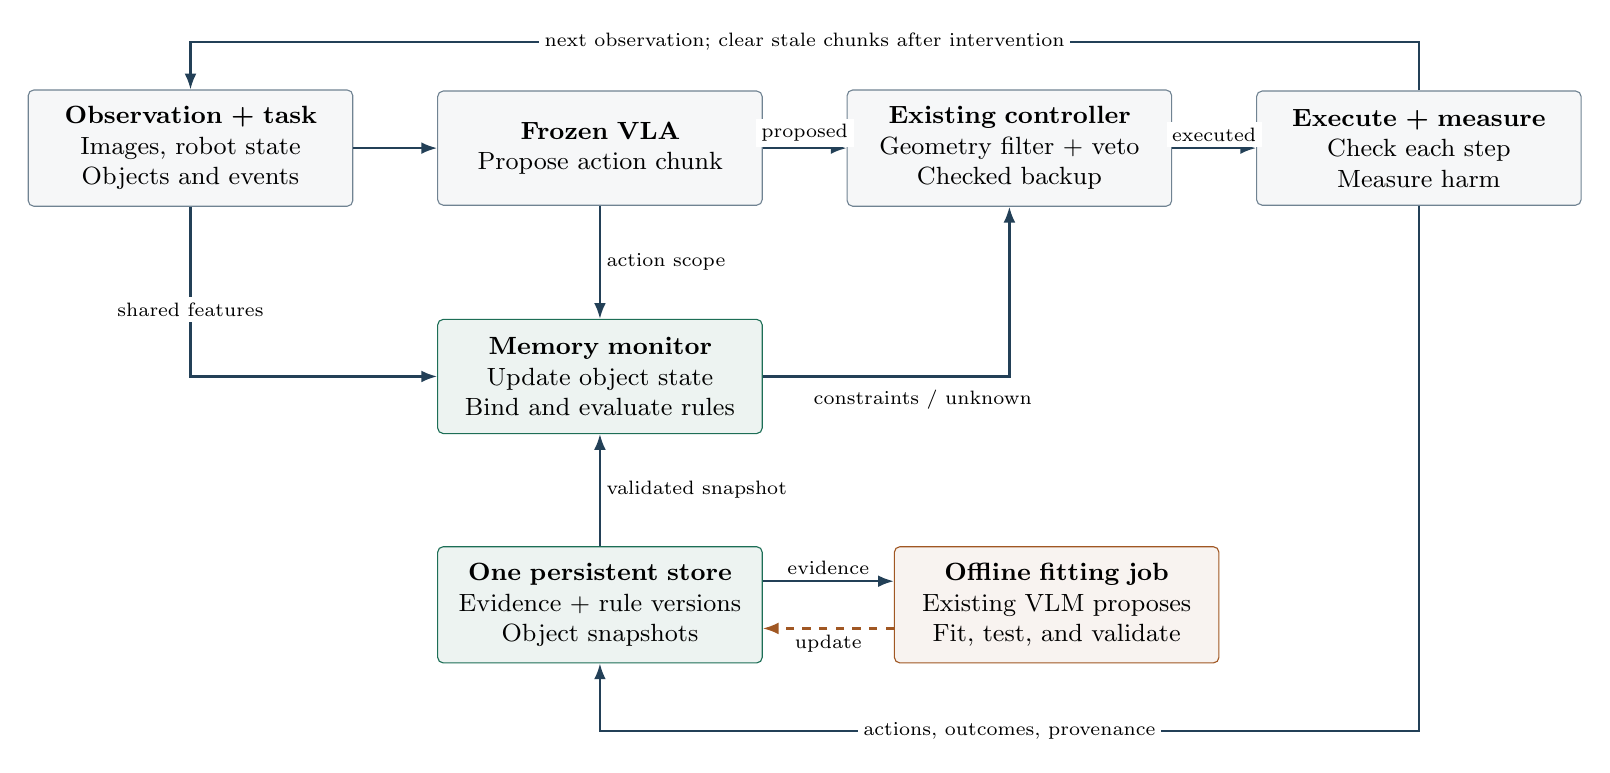
\begin{tikzpicture}[
 box/.style={rounded corners=2pt,draw=ink!65,fill=ink!4,align=center,text width=3.7cm,minimum height=1.45cm,inner sep=6pt,font=\small},
 flow/.style={-{Latex[length=2mm]},thick,draw=ink},
 update/.style={flow,dashed,draw=learn},
 lab/.style={font=\scriptsize,fill=white,inner sep=2pt}]
\node[box] (obs) at (0,0) {\textbf{Observation + task}\\Images, robot state\\Objects and events};
\node[box] (vla) at (5.2,0) {\textbf{Frozen VLA}\\Propose action chunk};
\node[box] (ctrl) at (10.4,0) {\textbf{Existing controller}\\Geometry filter + veto\\Checked backup};
\node[box] (robot) at (15.6,0) {\textbf{Execute + measure}\\Check each step\\Measure harm};
\node[box,draw=mem,fill=mem!8] (mon) at (5.2,-2.9) {\textbf{Memory monitor}\\Update object state\\Bind and evaluate rules};
\node[box,draw=mem,fill=mem!8] (store) at (5.2,-5.8) {\textbf{One persistent store}\\Evidence + rule versions\\Object snapshots};
\node[box,draw=learn,fill=learn!7] (fit) at (11,-5.8) {\textbf{Offline fitting job}\\Existing VLM proposes\\Fit, test, and validate};
\draw[flow] (obs)--(vla);
\draw[flow] (vla)--node[lab,above]{proposed}(ctrl);
\draw[flow] (ctrl)--node[lab,above]{executed}(robot);
\draw[flow] (obs.south)|-(mon.west);
\node[lab] at (0,-2.05) {shared features};
\draw[flow] (vla)--node[lab,right]{action scope}(mon);
\draw[flow] (mon.east)-|(ctrl.south);
\node[lab] at (9.3,-3.2) {constraints / unknown};
\draw[flow] (store)--node[lab,right]{validated snapshot}(mon);
\draw[flow] ([yshift=3mm]store.east)--node[lab,above]{evidence}([yshift=3mm]fit.west);
\draw[update] ([yshift=-3mm]fit.west)--node[lab,below]{update}([yshift=-3mm]store.east);
\draw[flow] (robot.south)--(15.6,-7.4)--(5.2,-7.4)--(store.south);
\node[lab] at (10.4,-7.4) {actions, outcomes, provenance};
\draw[flow] (robot.north)--(15.6,1.35)--(0,1.35)--(obs.north);
\node[lab] at (7.8,1.35) {next observation; clear stale chunks after intervention};
\end{tikzpicture}
}
\caption{Final proposed design. The new runtime component is the green memory monitor; fitting runs between deployments. Evidence, rule versions, and optional object snapshots share one logical store. Arrows from learning denote validated updates, never self-issued authority. The existing shield must still be checked for geometry, dynamics, and actuator correctness.}
\label{fig:system}
\end{figure}

\section{What the repository already does}
The inspection used the working tree on 11 October 2026 (root HEAD \code{75ca90d4}; submodules contain local changes). The live path is \code{fol_safety_filter/}, not the older 2D prototypes.

\begin{tabular}{p{0.29\linewidth}p{0.64\linewidth}}
\toprule
Observed component & Consequence for the proposed extension\\
\midrule
\code{filter.py:setup_episode} & Calls \code{self.kb.clear()}, grounds the scene, composes rules, and injects VLM-authored rules. Load persistent schemas separately from episode bindings.\\
\code{rule_composer.py} & Maps properties such as spillable, fragile, and hot to manually specified constraint templates. Learn applicability and parameters while retaining tested controller interfaces.\\
\code{kb.py} & Implements Boolean AND/OR/NOT over grounded calls. This is a limited formula evaluator, not a general quantified theorem prover. Unknown predicates and evaluation exceptions return False; replace this behavior in the new monitor.\\
\code{NovelPredicate} & Contains a grounding query and cached object Booleans. A name or cache entry is not an empirically learned predicate.\\
Memory proof of life & \code{experiments/safety_memory_poc} uses fixed handwritten rules and a scripted policy. It can test retention, but does not establish predicate invention or VLA transfer.\\
\bottomrule
\end{tabular}

The earlier September proposal separated several stores, an embedding index, a dependency graph, and recovery selection. This revision reduces the first implementation to one shared feature path, one monitor, one persistent evidence/library store, and an offline learning job. Raw clips may remain ordinary files referenced by the store. There is no need for multiple database services.

\section{Recent literature and what it changes}
This is a targeted review of primary sources from roughly October 2024 to October 2026, searched through 11 October 2026. It includes a September 2024 preprint published at ICRA 2025 as a directly relevant boundary case. Recent arXiv entries are treated as preprints unless a venue was verified. Results across different safety definitions are not directly comparable.

\small
\begin{longtable}{p{0.23\linewidth}p{0.35\linewidth}p{0.34\linewidth}}
\toprule
Work / date & Relevant contribution & Design implication\\\midrule\endhead
SafeVLA (2025) \cite{safevla} & Constrained policy learning explicitly trades task reward against safety cost. & A stronger training-based comparison if the memory-only method plateaus; initially avoid its rollout and optimization cost.\\
VLSA / AEGIS (Dec. 2025; revised July 2026) \cite{aegis} & Plug-and-play CBF constraints for VLA actions; introduces SafeLIBERO. & Reuse the existing control interface. A CBF does not establish the correctness of learned semantics.\\
RoboSafe (Dec. 2025) \cite{robosafe} & Executable predicate safety logic with short/long memory, retrospective temporal reasoning, and predictive contextual reasoning. & The closest conceptual overlap. ``Logic plus safety memory'' is already occupied. Avoid two online reasoning loops unless necessary.\\
CORE (Feb. 2026) \cite{core} & Grounds online VLM contextual safety reasoning into spatial safe sets enforced by CBFs. & Reasoning, grounding, and enforcement already exist together; persistent evidence-driven learning needs its own test.\\
SAFE (June 2025) \cite{safe} & A small detector uses VLA internal features to predict task failure. & Use shared frozen features as a cheap baseline. Relabel for physical harm: task failure and harm differ.\\
AnySafe (2025 preprint; ICRA 2026) \cite{anysafe} & Constraint-image-conditioned latent safety filtering, trained using a world model. & Demonstrates a credible non-symbolic alternative. The world-model dependency is too large for the first extension.\\
ShieldVLA (Sept. 2026) \cite{shieldvla} & Learned HJ-style safety critic gates VLA fine-tuning; VLM rubric scores provide supervision. & A learned critic is a serious alternative. Estimated safe regions and VLM targets still need independent validation.\\
FailBank (Sept. 30, 2026) \cite{failbank} & Runtime CBF feedback is retained and used for guarded LoRA policy updates; collection uses an observe-only teacher. & Persistent learning from shield feedback is established prior art. Our first design freezes the policy and learns the safety representation; real deployment keeps shielding active.\\
Multi-Link Safety Filtering (Sept. 30, 2026) \cite{multilink} & Multiple arm ellipsoids and sparse hazard tracking improve runtime shielding. & End-effector-only geometry and reset-only perception are inadequate. These are control requirements, not the proposed novelty.\\
Seeing the Invisible (Oct. 6, 2026) \cite{invisible} & Sensor-informed visual prompting steers a frozen navigation VLA around thermal/radiation hazards. & Some hazards require sensing; neither memory nor RGB semantics can recover an unobserved physical property reliably. Navigation evidence is adjacent to manipulation.\\
MemoryVLA (2025; ICLR 2026) \cite{memoryvla}; EventVLA (June 2026) \cite{eventvla} & Memory-conditioned action generation and selective retention of useful visual evidence. & Temporal context inside a policy differs from retaining learned safety rules between deployments. Both motivate a history-aware neural comparison.\\
SOMA (March 2026) \cite{soma} & Contrastive memory retrieval and offline consolidation adapt frozen VLAs through orchestration. & Textual or episodic retrieval must be a matched baseline. Retrieval and consolidation alone are insufficient novelty.\\
VisualPredicator (ICLR 2025) \cite{visualpred}; UniPred (Dec. 2025; revised Sept. 2026) \cite{unipred} & Learn grounded symbolic abstractions; UniPred couples foundation-model hypotheses with neural predicate learning. & Separate naming a predicate, learning its detector, and learning its consequences. Borrow frozen features and feedback, not the entire planner.\\
SkillWrapper (Nov. 2025; revised manuscript) \cite{skillwrapper} & Foundation-model-assisted predicate invention and abstraction learning from black-box skill interaction. & Predicate invention is established. Test history-dependent safety distinctions and evidence-efficient transfer specifically.\\
Santos et al. (ICRA 2025) \cite{feedback}; Du et al. (2026 manuscript) \cite{episodic} & Language-driven safety-set updates; episodic violations consolidated into semantic constraints. & Both online safety updates and remembered prohibitions have direct precedents.\\
LIBERO-Safety (June 2026) \cite{libsafe}; SafeVLA-Bench (2026) \cite{safebench} & Physical/semantic benchmark scenarios; task-aware temporal safety measurement separate from completion. & Measure harm independently, keep benchmark semantics distinct, and add a memory-required diagnostic suite.\\
\bottomrule
\end{longtable}
\normalsize

\textbf{Candidate contribution.} Learn a compact, object-bound safety state and conditional constraint from contrasted histories and incomplete intervention feedback, retain the validated rule, and transfer it to unseen objects during continuous VLA execution. This is a testable research claim, not a priority claim. RoboSafe already handles temporal predicates; SkillWrapper already invents predicates; FailBank already turns runtime feedback into persistent learning. The distinction must come from the learning protocol, measured transfer, and compute efficiency.

\section{Are predicates and first-order logic the right representation?}

\subsection{Why use predicates?}
A predicate gives a reusable name and argument structure to a measured distinction: $\mathrm{filled}(x)$ describes one object; $\mathrm{contactCandidate}(u,x,y)$ describes a proposed interaction. Its grounding function maps observations, geometry, or remembered evidence to true, false, or unknown. The name alone supplies no evidence. Learn the grounding from labeled examples and calibrate it on held-out objects.

Predicates are useful here because several restrictions can share the same detector and remembered fact. A learned fill estimate can condition tilt and speed limits; an exposure state can be reused with several protected surfaces. Object arguments make it possible to inspect which binding caused an intervention. They also separate a perception error from an incorrect restriction during debugging. These are engineering benefits to test through detector reuse, sample efficiency, and intervention accuracy.

The cost is an information bottleneck. A Boolean can hide uncertainty or discard a continuous quantity needed for control. Keep probabilities for calibration, an explicit unknown value for runtime decisions, and numerical geometry for the controller. Do not force every latent feature into a named concept. If a small action-conditioned predictor performs better with the same data and budget, use it.

\subsection{What the cited paper establishes}
Brunke et al.'s \emph{Semantically Safe Robot Manipulation: From Semantic Scene Understanding to Motion Safeguards} is the supplied IEEE paper (RA-L 2025, DOI 10.1109/LRA.2025.3553046) \cite{brunke}. The author manuscript's Sections IV-B to IV-D describe LLM-generated semantic context for a manipulated object: object/relation pairs, caution settings, and rotation settings. These configure spatial CBFs, approach behavior, and a softened rotation objective. Evaluation includes teleoperation and learned diffusion policies. It is direct evidence that useful semantic safeguards can be implemented without a general FOL inference engine.

Its object-pair representation already captures relations. Consequently, adding object variables or writing a safety condition in logical notation is insufficient as a contribution over this paper. The proposed extension must demonstrate learned applicability from outcome evidence, retained history-dependent state, and reuse across deployments. None of these benefits follows merely from choosing FOL. The comparison below therefore includes a direct constraint-mapping system with the same learned predicates and memory.

\subsection{Why use a restricted first-order rule schema?}
Predicates and FOL are different levels of description. A predicate is a property or relation; FOL supplies variables, connectives, and quantification for statements involving predicates. A grounded predicate evaluator can also combine conditions in ordinary code. Conjunction, memory retention, and action vetoes do not require a theorem prover.

The proposed use of first-order notation is a compact storage format for a learned conditional restriction. For example, over the finite set $O_t$ of tracked objects,
\[
\forall x,y\in O_t:\quad
\mathrm{exposed}_t(x)\land\mathrm{protected}(y)
\land\mathrm{contactCandidate}(u,x,y)
\Rightarrow\mathrm{veto}(u).
\]
The repeated variable $x$ requires the exposed object to be the object about to contact $y$. With two tools, exposure of tool A must not prohibit an otherwise safe contact by clean tool B. A single schema can be rebound to new tools and surfaces, avoiding a separate learned table entry for each object ID. Its possible advantage is parameter sharing and a compact, revisable representation of conditions. A procedural pair loop or a shared neural pair model can provide the same binding and sharing; logical syntax has no exclusive claim to either.

Use a function-free, nonrecursive rule schema with at most two object variables and three antecedent literals. Instantiate it with finite loops; do not add a solver, recursive proof search, existential object generation, or a planner. Runtime truth is three-valued because perception can be unknown, so this is not unrestricted classical FOL reasoning. Temporal state comes from the learned event update, not from first-order quantification. With $R$ rules and $N$ tracks, naive pair evaluation is $O(RN^2)$, or $O(RN)$ when one role is the held object. Share predicate evaluations and use only conservatively justified relevance pruning.

\subsection{Answering the predicate-only objection}
A reviewer is right if ``predicates only'' means learned predicates with a direct conditional mapping to the same constraints. Such a system may already implement an equivalent rule. We should not claim that FOL is necessary, more physically safe, or more expressive than an equivalent finite program. The narrower hypothesis is that storing learned conditions as short schemas improves transfer, revision, or data efficiency enough to justify the representation.

Test this with the same detectors, remembered state, outcome data, controller, calibration budget, and fixed physical limits:
\begin{enumerate}
\item Direct predicate-to-constraint mapping, including a Brunke-style object-pair context interface. Permit conjunctive conditions and conditional parameter selection; restricting this baseline to isolated unary triggers would weaken it unfairly.
\item A small shared object-pair risk head over the same predicate probabilities and memory, with its output mapped to the same constraint/veto interface. Pool pair decisions consistently when object counts change.
\item The proposed learned bounded schemas, instantiated on the same object pairs.
\end{enumerate}
Include safe counterexamples, unseen object pairs, swapped roles, and scenes with additional distractor objects. Evaluate matched safety/completion trade-offs, labels needed, latency, and the cost of revising a restriction without damaging old cases. A single hidden-fill cup task can establish a memory benefit; it cannot establish a need for FOL. Run a separate two-tool/two-surface binding diagnostic to test relational reuse. If direct mappings match the schema learner, retain the simpler implementation and describe the contribution as learned safety memory. If both implementations encode the same function, treat their comparison as an implementation check, not a scientific distinction.


\begin{tabular}{p{0.22\linewidth}p{0.36\linewidth}p{0.34\linewidth}}
\toprule
Representation & Strength & Limitation / decision\\\midrule
Retrieved text or episodes & Immediate addition; flexible language; almost no training. & Similarity is not applicability; prompts may be ignored. Keep as baseline and proposal context.\\
Bounded relational rules & Reuse across object bindings; inspectable exceptions; direct control mapping. & Requires reliable concepts. Recommended initial interface, with uncertainty retained.\\
General FOL / PDDL & Rich quantification and compositional planning. & More search and specification machinery than needed for local action constraints. Defer.\\
Temporal logic / automata & Represents order, duration, and persistence explicitly. & General formula synthesis adds complexity. Begin with one generic set/reset memory bit; use STL mainly for evaluation.\\
Small recurrent risk head & Learns features/history jointly; one numerical predictor; scales with data. & Can miscalibrate or forget; weaker explicit transfer and debugging. Implement as the principal challenger.\\
World model + planning & Predicts alternative futures and delayed effects. & Expensive training, rollout latency, and model exploitation. Add only if short-horizon monitoring demonstrably fails.\\
\bottomrule
\end{tabular}

The initial rule has the form
\[
\underbrace{C_\phi(x_t,z_t,o_1,\ldots,o_k)}_{\text{grounded context and memory}}
\wedge\underbrace{A(u,o_1,\ldots,o_k)}_{\text{proposed interaction}}
\;\Rightarrow\; \underbrace{u\in\mathcal U_{\eta}(x_t)}_{\text{control constraint}},\qquad k\leq2.
\]
Here $x_t$ contains sensed geometry and shared visual features, $z_t$ contains remembered state, and $u$ is a candidate action. Start with at most three antecedent literals, unary/binary predicates, no recursive inference, and an allowlisted consequence: clearance, speed bound, orientation bound, or veto. This is a bounded conditional rule language, with implicit iteration over relevant tracked objects. Its expressiveness limits must be reported.

Probabilities are useful for detectors, but multiplying predicate probabilities would assume unjustified independence. First calibrate each detector, retain three-valued truth (true/false/unknown), and evaluate rule conditions conservatively. Later fit an action-conditioned risk head directly if joint uncertainty is important. Continuous geometry stays continuous; do not turn every distance into a named Boolean.

\section{Learning predicates, learning rules, and retaining them}
\subsection{A single evidence record}
Use an append-only JSONL ledger and versioned JSON/NPZ library snapshots initially. One coordinator writes the library; parallel Slurm workers write independent shards merged offline. This avoids concurrent writes to a shared database. A local SQLite database is optional only if indexing becomes necessary.

\begin{lstlisting}
Evidence = {
  episode_id, physical_reset_id, object_track_ids, timestamps,
  observation_clip_ref, features_ref, sensed_geometry,
  proposed_action, executed_action, intervention_reason,
  outcome, outcome_horizon, outcome_source, censored,
  policy_version, detector_version, library_version, seed
}
Rule = {
  id, roles, detector_ids, condition, state_update,
  action_scope, constraint_type, constraint_parameters,
  validity_domain, support_ids, contradiction_ids,
  calibration_report, regression_report, version, status
}
\end{lstlisting}

Outcomes include actual harm, observed safe completion within a stated horizon, and unresolved outcomes. Task failure alone is not harm. A blocked nominal action has no observed outcome; a successful filtered rollout labels the executed action only. Simulator counterfactuals are separate evidence with their own provenance. They are useful only to the extent that the simulator models the relevant hazard.

\subsection{What exactly is learned?}
\textbf{Grounding.} For each candidate concept, train a linear/logistic head on frozen object or object-pair crop features plus measured geometry. Use a frozen vision encoder already exposed by the current stack; if policy internals are unavailable, cache features from one existing VLM vision encoder. Role-specific crops and geometric differences are required: a global scene token alone can learn spurious task identity. Perception confidence comes from labeled validation data, not the VLM's stated confidence.

\textbf{Vocabulary.} A VLM can propose at most a small batch of candidate distinctions from matched safe/unsafe clips and existing counterexamples. Its outputs are hypotheses. Candidate names never become active rules automatically. Select a concept only when its detector is learnable and adding it improves held-out action-outcome prediction. Freeze discovery prompts and record the candidate budget. An ablation using anonymous learned features tests whether language naming is useful.

\textbf{Temporal state.} If comparable current observations and actions have inconsistent outcomes, inspect preceding events. Start with a generic finite-state template: set on event $e^+$, retain, clear on verified event $e^-$. Search over learned event detectors and object bindings. Unknown evidence remains unknown; disappearance is not clearance. This discovers an instance within a declared grammar, not arbitrary hidden physics. Add counters/decay or a small GRU only if the simple template fails on held-out histories.

\textbf{Rule and numerical boundary.} Enumerate shallow conjunctions over grounded concepts, action type, and optional memory state. Fit consequences and thresholds using controlled simulation or measured trials: for example, compare tilt limits for full and empty containers. A depth-limited tree or beam search is sufficient; use one implementation. Keep a Pareto set balancing missed hazards, unnecessary restrictions, and description length:
\[
J=\widehat L_{\rm hazard}+\beta\widehat L_{\rm overrestriction}
  +\lambda\bigl(\#\text{literals}+\#\text{new states}\bigr).
\]
Evaluate losses on appropriately labeled data; do not impute outcomes for blocked actions. Select complexity on development data, then calibrate on a separate split. Error weights reflect the declared hazard severity. Neither $J$ nor minimum description length is a safety proof.

\subsection{A concrete learning loop}
\begin{enumerate}
\item Collect matched safe and unsafe outcomes in simulation, varying object appearance, action, and hazard state independently. Start from the existing baseline/filter traces where their sensors are trustworthy.
\item Find repeated errors or history aliasing. Query the existing VLM offline for candidate concepts/events; include successful counterexamples and candidate exceptions.
\item Fit the shared-feature detector heads. Reject candidates supported only by object names, task IDs, or unavailable sensors.
\item Fit shallow rules and, only where needed, the generic memory update. Test competing explanations with simulator interventions that change one variable at a time. Keep deterministic seed/state matching.
\item Validate complete complete perception, memory, rule, and controller chains on separate scenes and histories. Require improvement in safe task completion and no unacceptable increase in measured harm under predeclared confidence bounds. Insufficient data leaves a candidate inactive.
\item Publish a versioned library snapshot between evaluation batches. Log contradictions, retain regression pairs, and roll back or narrow scope when later evidence invalidates a rule. Refit from retained evidence to reduce forgetting.
\end{enumerate}

Unsafe tests belong in simulation or a physically bounded test setup. Deployment data alone often cannot identify the risk of actions that the shield always blocks: no amount of reweighting fixes zero action coverage. Prefer targeted simulator trials or qualified feedback over unshielded exploration.

\subsection{Pseudocode: learn and commit a library}
Algorithm 1 runs between deployments. A library snapshot contains detector weights, calibration, state updates, rule schemas, controller parameters, and evidence IDs. Hyperparameters and acceptance thresholds are fixed before evaluation. The immutable final test set is never an input to fitting or acceptance.

\begin{lstlisting}[caption={Algorithm 1. Offline learning and persistent reuse},basicstyle=\ttfamily\footnotesize]
def learn_library(ledger, old_library, fixed_limits):
    # Split by whole episode, object, scene, and history family.
    train, dev, calibration, acceptance = acquisition_splits(ledger)
    train = label_executed_actions_only(train)
    # Unexecuted proposals stay censored unless independently tested.
    concepts = propose_bounded_candidates(train, old_library)
    heads = fit_heads(frozen_features(train), concepts)
    heads = select_learnable_heads(heads, dev)
    states = fit_set_retain_reset_updates(train, heads)
    candidates = enumerate_rules(heads, states,
                                 max_objects=2, max_literals=3)
    candidates = fit_allowed_consequences(candidates, train,
                                         fixed_limits)
    candidate = select_by_harm_overrestriction_complexity(
                    candidates, dev, include=old_library)
    candidate = calibrate_truth_and_unknown(candidate, calibration)
    report = evaluate_complete_chain(candidate, acceptance,
                                    retained_regression_cases())
    if not passes_predeclared_gates(report):
        archive_inactive(candidate, report)
        return old_library
    snapshot = package(candidate, report, evidence_ids=ledger.ids,
                       encoder_version=frozen_encoder.version)
    atomic_commit(snapshot)  # Single writer; preserve rollback version.
    return snapshot
\end{lstlisting}

Predicate labels come from independently measured attributes/events or separately verified annotations. Outcome labels alone may admit several equally predictive concept decompositions; a useful unnamed feature is not automatically the claimed semantic predicate. Insufficient grounding labels leave a proposed named detector inactive. Fit memory updates by replaying complete histories. Acceptance data must be renewed or protected from repeated adaptive reuse; repeatedly tuning against a fixed acceptance set leaks information.

\subsection{Reuse and forgetting}
A schema such as ``an exposed tool must not contact a protected surface'' is rebound to new objects; a fact such as ``track 17 is exposed'' is tied to a physical identity and reset history. Rule schemas persist between episodes. Facts persist only when identity and physical continuity are justified. A new benchmark episode is not evidence that a real tool became clean.

For the initial small library, scan every validated rule applicable to the action and object roles. This is cheaper to implement and easier to audit than semantic top-$k$ retrieval. Embedding search may later retrieve training examples, but must not omit a known active constraint. A library snapshot includes detector weights, feature-encoder version, units, calibration, and supporting/contradicting evidence. Evicting duplicate examples must preserve rare hazards and exceptions. A changed encoder invalidates old feature-based calibration until retested.

\section{Worked example: discovering an exposure memory}
Use a harmless simulated marker-transfer mechanism, not an unsupported claim about real biological contamination. An independent hidden simulator ledger determines transfer; its state is never included in runtime observations. Generic contact observations are available with uncertainty.

\begin{enumerate}
\item In history A, a tool touches a marked source. In history B, the same-looking tool does not. The final RGB views are matched. Both tools are then moved toward the same kind of protected surface.
\item The measured transfer outcomes differ across repeated, controlled trials. A frame-only classifier cannot separate the cases if the observations are truly aliased. Longer observation history can.
\item Candidate explanations include color, tool identity, previous source contact, and elapsed time. Matched object swaps and same-action tests reject color/identity shortcuts. The selected state is provisionally named \code{exposed(x)}.
\item Fit event detectors and select the persistence/reset template. Learn the contact-conditioned restriction. Effective cleaning and ineffective wiping are separate tests; neither the word ``clean'' nor elapsed time automatically clears the state.
\item At deployment, the state updates from observed events; a rule blocks predicted contact with the protected surface. It allows unrelated motion and allows the interaction after verified reset. New tool/surface bindings reuse the schema.
\end{enumerate}

A deterministic illustration of the selected state machine is
\[
z_{t+1}(x)=
\begin{cases}
1 & \text{verified source-contact event},\\
0 & \text{verified effective-reset event, with no simultaneous exposure},\\
z_t(x) & \text{otherwise, with reliable identity and observation},\\
? & \text{ambiguous identity or potentially missed relevant event}.
\end{cases}
\]
The learned rule is $z_t(x)=1\ \wedge\ \mathrm{contactCandidate}(u,x,y)\ \wedge\ \mathrm{protected}(y)\Rightarrow\mathrm{veto}(u)$. An unknown relevant antecedent triggers observation or a validated backup, not unconditional free motion. \code{contactCandidate} is obtained from sensed geometry, calibrated action scaling, and a short swept-motion check; it is not a guessed action label. Test the swept volume of the held object as well as the arm.

If the experiment starts with the exposure detector, reset rule, and contact prohibition already specified, it measures memory retention only. To claim discovery, withhold at least the state choice and rule condition; train the event grounding from separate data; report each supplied primitive. To claim transfer, hold out object instances, layouts, and event compositions. If reset tests provide no evidence, retain uncertainty rather than inventing a cleaning rule.

\section{Where the naive design fails, and the revision}
\small
\begin{longtable}{p{0.23\linewidth}p{0.32\linewidth}p{0.37\linewidth}}
\toprule
Failure & Why a simple cache/rule system fails & Minimal improvement in the final design\\\midrule\endhead
Hallucinated predicate & Plausible VLM text becomes a confident rule. & Require labeled detector evaluation and held-out behavioral evidence before activation.\\
Unknown treated as false & A missing hot/exposed detection silently removes protection. & Three-valued evaluation; unknown cannot prove a relevant hazard absent. Fix negation semantics as well.\\
Intervention censoring & A blocked action is mislabeled unsafe, or a corrected success labels the original action safe. & Store proposed/executed actions separately; censor blocked outcomes; obtain independent diagnostic evidence.\\
Shortcut learning & All dangerous objects share color, task ID, or category. & Matched scene/action pairs and object/layout splits; test counterexamples that break correlations.\\
Incorrect attribution & A failure is blamed on the last visible event. & Use controlled action/history interventions; retain multiple hypotheses until distinguished.\\
Overgeneralization & ``Never touch cups'' prevents both spills and useful work. & Include safe contacts and task-required exceptions; optimize safe completion, not zero motion.\\
Stale fact or identity swap & A rule remains correct but is applied to the wrong tool. & Bind facts to physical identity and reset provenance; uncertain reassociation produces unknown.\\
Unobservable physical state & RGB is assumed to reveal temperature or contamination. & Require a sensor, verified event model, or uncertainty. Memory cannot supply missing evidence.\\
Unsupported controller mapping & A semantic risk is converted into an arbitrary larger sphere. & Compile only supported consequences; use an explicit veto/backup for unsupported interactions.\\
Action chunk becomes unsafe & Only the first point or stale reset geometry was checked. & Check swept motion and filter each executed step; invalidate the chunk after correction or new evidence.\\
Arm or held-object collision & End-effector clearance hides elbow/object contact. & Validate relevant body and held-object geometry; limit claims to covered surfaces.\\
Contradictory constraints & A QP is infeasible or oscillates between restrictions. & Precedence for fixed physical limits; detect infeasibility; use a validated backup rather than silent relaxation.\\
Stop is itself unsafe & Zero velocity can drop a load or leave heating active. & Declare a state-dependent backup controller and its applicability. If none is available, no safety claim covers that state.\\
Memory poisoning / drift & Repeated mistaken judgments reinforce a rule or obsolete calibration. & Source-tag evidence, keep measured labels distinct from judgments, version updates, replay old cases, and quarantine conflicts.\\
No task progress & Frozen VLA repeatedly proposes the same vetoed action. & Clear stale chunks, make one bounded replan/observation attempt, then terminate safely. Add recovery learning only if this is the dominant error.\\
Vacuous benchmark success & A dead or absent safety predicate reports perfect safety. & Independent per-step harm scorer, including terminal steps, with deliberate positive controls.\\
\bottomrule
\end{longtable}
\normalsize

This failure analysis changes the design in three substantive ways: memory contains evidence and validity, conditions can be unknown, and the controller checks the action actually executed. None requires another foundation model or an online agent hierarchy.

\clearpage
\section{Final runtime and control boundary}
At episode setup, load a frozen validated library snapshot, establish object identities, and initialize beliefs from justified observations or physical continuity. Keep learned schemas outside \code{kb.clear()}. At every execution step:

\begin{lstlisting}[caption={Algorithm 2. Runtime monitoring with a frozen library},basicstyle=\ttfamily\footnotesize]
library = load_validated_snapshot()  # Survives process/episode resets.
belief = initialize_from_verified_continuity_or_unknown()
pending, previous_obs = [], UNAVAILABLE
for observation, timestamp in sensor_stream():
    # Outcomes mature after execution; unresolved records stay censored.
    mature_outcome_records(pending, observation, timestamp)
    tracks, features, geometry = observe_and_track(observation)
    events = library.detect_events(features, geometry, previous_obs)
    belief = library.update_state(belief, events, tracks,
                                  verified_physical_reset())
    u_nom = next_step_of_frozen_VLA_chunk(observation)
    bindings = all_relevant_bindings(library, tracks, u_nom)
    truth = library.ground(features, geometry, belief, bindings)
    constraints, unknown = evaluate_three_valued(library, truth, u_nom)
    u = NONE
    if fresh_enough(timestamp) and not relevant_unknown(unknown):
        u = existing_filter(u_nom, constraints, fixed_physical_limits)
        # Correction can create a new contact: rebind and recheck it.
        if u is NONE or not passes_all_rules_and_swept_checks(
                                 u, library, belief,
                                                tracks, geometry):
            u = NONE
    if u is NONE or deadline_missed():
        u = validated_applicable_backup_or_NONE(current_state())
    if u is NONE:
        declare_uncovered_state_and_handoff()
        break  # Outside the declared safety guarantee.
    execute(u)
    pending.append(log_proposal_execution(u_nom, u, truth,
                   library.version, outcome=UNRESOLVED))
    if u != u_nom or relevant_event(events):
        discard_remaining_action_chunk()
    previous_obs = observation
flush_pending_as_unresolved_if_horizon_incomplete(pending)
\end{lstlisting}

Event detection returns unknown on the first tick where it needs an observation pair. Failed or timed-out solver calls return \code{NONE}; the final action check rejects unknown as well as violated conditions. Missing tracks or geometry also propagate unknown. Outcome collection is a separate observer: privileged simulator labels may enter the evidence ledger after execution but never the runtime predicate features. A backup is checked under its own validated applicability conditions. Handoff is a declared failure of coverage; it must not be counted as a safe completion. Each control tick uses a fixed snapshot, and a newly committed library is loaded only at a deployment boundary.


In a discrete implementation, the geometric component may solve
\[
\min_{u\in\mathcal U}\|u-u_{\rm nom}\|_W^2
\quad\text{s.t.}\quad
h_j(\widehat f(x_t,u))\geq(1-\alpha_j)h_j(x_t)+m_j,
\]
for applicable geometric constraints. This is a QP only when the implemented constraints are affine in $u$ (or suitably linearized); otherwise it is a nonlinear program. Here $m_j$ covers a justified bound on relevant model/measurement errors. Arbitrary semantic predicates do not become valid CBFs by substitution. With linearization, discretization, uncertain perception, moving obstacles, or incomplete geometry, the actual controller needs its own validity analysis and empirical checks.

Use three-valued logic: NOT unknown remains unknown; AND is false if any operand is known false, true only if all are known true, and unknown otherwise. Rule activation depends on the action being relevant, so an uncertain property of a distant uninvolved object need not halt everything. Do not allow learned rules to loosen fixed joint, workspace, or actuator limits.

\textbf{Timing.} The CPU monitor/filter runs at the existing execution rate. The shared visual path runs at the fastest rate demonstrated by profiling; full VLM generation is event-triggered or offline. Set an observation-age budget and geometry inflation from measured latency and hazard speed. If these assumptions fail, use the backup. A desired 20 Hz monitor leaves 50 ms per tick; a target of under 5 ms for the added CPU monitor is an engineering target, not a measured result. Never put an unpredictable network model call in the hard deadline path.

\section{PSC capacity and a bounded experiment budget}
\textbf{Verified locally on 11 October.} \code{sinfo} exposes \code{GPU-shared} with V100-16, V100-32, L40S-48, and H100-80 GPU types. \code{sacctmgr} lists \code{cis240028p} for this user. A 48-hour, one-H100 \code{sbatch --test-only} request was accepted; this submits no workload. The repository's Ocean directory name \code{cis250185p} is not the Slurm account. This check establishes request compatibility, not remaining allocation, immediate availability, or a guaranteed maximum walltime.

PSC documents 32/48/80 GB per GPU for the proposed V100/L40S/H100 options, and current GPU-hour charging factors of 1/1/2 SU respectively \cite{psc}. Choose the device by measured end-to-end time per SU and software compatibility. H100 wins on SU cost only if its relevant workload is more than twice as fast as the one-SU alternative. Queue delay also matters. Do not assume advertised node inventory is free capacity.

\begin{tabular}{p{0.28\linewidth}p{0.29\linewidth}p{0.35\linewidth}}
\toprule
Work & Initial resource choice & Scope / caveat\\\midrule
Rule search, regression, metadata & CPU within an allocated job & No VLA backpropagation. Batch this work with feature or rollout jobs if a CPU-only allocation is unavailable.\\
Feature extraction and small heads & One V100-32 or L40S-48 & Reuse cached crops/features; check kernels and precision on V100.\\
Frozen OpenVLA-OFT rollout & One V100-32, following existing scripts & Actual memory/latency need a pilot with this model and image configuration.\\
Joint local VLA + VLM & One H100-80 as first profiling target & Two 7B models have roughly 28 GB of FP16 weights alone; activations, vision towers, caches, and simulator overhead determine fit.\\
Optional adapter comparison & One H100-80, after memory result & Small head first; LoRA or a larger latent model only after a measured bottleneck.\\
\bottomrule
\end{tabular}

\textbf{Storage arithmetic.} At 100,000 retained event examples, 1,024-dimensional FP16 embeddings use about 205 MB per embedding stream. Two compressed 200 KB views per event use about 40 GB before additional clips. These are planning assumptions; record actual sizes. Store every episode's metadata and sampled successes, plus failure/event windows. Avoid keeping every video frame solely to support a tiny rule library.

\textbf{Rollout budget, explicitly an estimate.} Run a 20-episode pilot to measure walltime, peak VRAM, feature cost, and model-startup time. Then a first board can use 12 scenario variants $\times$ 10 paired seeds $\times$ 6 methods = 720 scored episodes. If one allocated GPU averages 120 seconds per episode, this is 24 GPU-hours; at 300 seconds it is 60 GPU-hours. Add a provisional 20 GPU-hours for data collection, feature extraction, fitting, and diagnostics, then 20\% contingency: approximately 53 to 96 GPU-hours, or 106 to 192 SU if all work uses H100. Acquisition phases in paired memory episodes must be included in the measured episode time or budgeted separately. These are not measurements or confirmation of available SU balance.

Start with two concurrent single-GPU shards, checkpoint after each episode, and scale concurrency only if the allocation and queue allow. Use \code{GPU-shared}, not a whole node for a one-GPU job. Cache models on Ocean, stage active files to node-local scratch when available, and merge results after completion. Keep \code{env_seed} identical across paired methods. GPU jobs, simulation, and substantial fitting belong under Slurm; this proposal launches none.

\section{Experiments that can reject the design}
\subsection{First fix the measurement boundary}
The repository's \code{docs/code_review_findings.md} reports an always-false robot-contact path, absent affordance constraints, duplicate-cost-key loss, and missing terminal-step costs in the local LIBERO-Safety evaluation path. Do not train safety labels or claim improvements from those columns without an independent audited scorer. Inject known contacts and noncontacts to test the scorer, and report sensor-unavailable checks as N/A.

SafeLIBERO completion can coexist with collisions; LIBERO-Safety's violation termination changes its success semantics. Report native metrics separately. Add common independently measured outcomes: any-harm rate, severity, task completion, and \emph{safe completion} (completion with no measured violation). SafeVLA-Bench's separation of success and safety is useful here \cite{safebench}.

\subsection{A memory-required diagnostic, then benchmark transfer}
Use three hazard families with four variants each: remembered exposure, remembered fill/spill state, and persistent damage/load sensitivity. These are proposed instrumented simulation tasks, not claims about existing benchmark coverage. Include visible controls, hidden-state variants, valid reset cases, and misleading/ineffective-reset cases. The independent hazard ledger must be physically or procedurally specified, audited, and inaccessible to the monitor. Privileged state may supply training labels but must not enter test features.

Split entire object instances, scenes, and history templates between train/development/calibration/test; adjacent frames from one episode must never cross splits. A separate continual evaluation freezes the library during each test batch, then permits updates from a labeled acquisition batch before the next deployment. Hold a final immutable transfer set. Keep true physical continuity separate from statistical independence across trials.

\textbf{Six primary methods, same VLA, observations, and geometric backbone:}
\begin{enumerate}
\item Current stateless filter.
\item Matched text/episode retrieval with a fixed online token and call budget.
\item Learned predicates/rules using current observations only.
\item Full proposed learned rule memory.
\item Small GRU action-conditioned harm predictor on the same shared features/history; same veto interface and data.
\item Oracle safety state/rules with the same controller, explicitly privileged, as a diagnostic ceiling.
\end{enumerate}

The three-method predicate-versus-schema panel in Section 4 is a separate follow-up after the memory effect is established; its rollouts are additional to the six-method budget above. Run a targeted deletion panel for method 4: erase the object fact, erase the learned schema, and retain everything. This separates within-history memory, persistent rule reuse, and current-image prediction. A hand-written memory rule is an additional diagnostic to separate learning error from retention error. Match model-selection effort and include offline compute in every method's cost.

Report safe completion and harm at matched intervention rates or matched task-completion levels, alongside the full trade-off curve. Also report false vetoes on independently verified safe alternatives, unknown/abstention frequency, predicate calibration, new-object transfer, old-hazard forgetting, support count per rule, and p50/p95/p99 latency. Paired episode bootstrap or paired tests should respect task/seed clustering. A few favorable episodes do not establish rare-event safety: with zero violations in $n$ independent comparable trials, the one-sided 95\% binomial upper bound is $1-0.05^{1/n}$, about 3\% at $n=100$. Reused histories and correlated trials weaken that interpretation.

\subsection{Decision gates}
\begin{enumerate}
\item If ground-truth memory does not improve hidden-state cases, repair the benchmark or controller before learning.
\item If hand-written memory works but learned memory fails, separate detector error, state-update error, and rule-induction error using oracle swaps.
\item If the GRU matches or exceeds rule memory at comparable data, latency, and retention, use the GRU as the primary monitor; keep predicates only as optional explanations. Require explanations to be faithful before exposing them as operational rules.
\item If memory raises safety only by stopping, reject the claimed improvement. Diagnose recoverable veto loops before adding a bounded recovery interface.
\item If larger data budgets improve the latent model faster, report that scaling result and reduce symbolic constraints on representation. If rules transfer with less data, report the regime where their bias pays off.
\end{enumerate}

\section{Implementation sequence and final scope}
\textbf{First implementation.} Add \code{safety_memory.py} for evidence and snapshots, \code{memory_monitor.py} for role binding/uncertainty/state, and one \code{learn_safety_memory.py} job for feature heads and bounded rule search. These are proposed filenames, not existing implementations. Modify episode setup to preserve the library, route monitor constraints into \code{cbf_mapper.py}, and log nominal/executed actions in the evaluation driver. Keep the existing VLM as an offline hypothesis proposer. Start with one hazard family and one backbone (OpenVLA-OFT); test $\pi_{0.5}$ only after the memory effect is established.

\textbf{What is fixed.} Sensors, object tracking interface, generic set/reset grammar, supported controller actions, hard physical limits, and outcome definitions. \textbf{What is learned.} Candidate distinctions selected from evidence, detector weights, applicable relational conditions, temporal event bindings, and constraint parameters within validated controller limits. \textbf{What is remembered.} Grounded current facts when continuity is justified, learned schema versions, and the evidence needed to revise them.

The final system is a frozen VLA with a learned memory monitor feeding the existing safety controller. It can acquire and reuse compact safety knowledge without retraining the base policy. Experiments must establish whether it improves adaptation and transfer under partial observability. Unmodeled hazards, incorrect perception, identity errors, insufficient action coverage, and an invalid backup remain failure modes; the design makes them measurable rather than claiming to eliminate them.

\clearpage
\begin{thebibliography}{99}
\bibitem{safevla} Zhang, Borong et al.. \emph{SafeVLA: Towards Safety Alignment of Vision-Language-Action Model via Constrained Learning}. 2025/03/05.  \url{https://arxiv.org/abs/2503.03480}.
\bibitem{aegis} Hu, Songqiao et al.. \emph{VLSA: Vision-Language-Action Models with Plug-and-Play Safety Constraint Layer}. 2025/12/09.  \url{https://arxiv.org/abs/2512.11891}.
\bibitem{robosafe} Wang, Le et al.. \emph{RoboSafe: Safeguarding Embodied Agents via Executable Safety Logic}. 2025/12/24.  \url{https://arxiv.org/abs/2512.21220}.
\bibitem{core} Ravichandran, Zachary et al.. \emph{Contextual Safety Reasoning and Grounding for Open-World Robots}. 2026/02/23.  \url{https://arxiv.org/abs/2602.19983}.
\bibitem{safe} Gu, Qiao et al.. \emph{SAFE: Multitask Failure Detection for Vision-Language-Action Models}. 2025/06/11.  \url{https://arxiv.org/abs/2506.09937}.
\bibitem{anysafe} Agrawal, Sankalp et al.. \emph{AnySafe: Adapting Latent Safety Filters at Runtime via Safety Constraint Parameterization in the Latent Space}. 2025/09/23.  \url{https://arxiv.org/abs/2509.19555}.
\bibitem{shieldvla} Tayal, Manan et al.. \emph{ShieldVLA: Feasibility-Aware Safety Alignment for Vision-Language-Action Models}. 2026/09/02.  \url{https://arxiv.org/abs/2609.13231}.
\bibitem{failbank} Cui, Mingyue et al.. \emph{Learning from Runtime Feedback through Failure-Bank Self-Evolution for Vision-Language-Action Models}. 2026/09/30.  \url{https://arxiv.org/abs/2609.39820}.
\bibitem{multilink} Agarwal, Yatharth et al.. \emph{Multi-Link Safety Filtering for VLA Policies Around Moving Hazards}. 2026/09/30.  \url{https://arxiv.org/abs/2609.40007}.
\bibitem{invisible} Son, Hojoon et al.. \emph{Seeing the Invisible: Physics-Guided Visual Prompting for Temperature- and Radiation-Aware VLA Navigation}. 2026/10/06.  \url{https://arxiv.org/abs/2610.07558}.
\bibitem{memoryvla} Shi, Hao et al.. \emph{MemoryVLA: Perceptual-Cognitive Memory in Vision-Language-Action Models for Robotic Manipulation}. 2025/08/26.  \url{https://arxiv.org/abs/2508.19236}.
\bibitem{eventvla} Yang, Ganlin et al.. \emph{EventVLA: Event-Driven Visual Evidence Memory for Long-Horizon Vision-Language-Action Policies}. 2026/06/18.  \url{https://arxiv.org/abs/2606.20092}.
\bibitem{soma} Li, Zhuoran et al.. \emph{RoboHarness: A Memory-Augmented Policy Harness for Vision-Language-Action Model Robustness via In-Context Adaptation}. 2026/03/25.  \url{https://arxiv.org/abs/2603.24060}.
\bibitem{unipred} Wang, Qianwei et al.. \emph{Unifying Deep Predicate Invention with Pre-trained Foundation Models}. 2025/12/19.  \url{https://arxiv.org/abs/2512.17992}.
\bibitem{skillwrapper} Yang, Ziyi et al.. \emph{SkillWrapper: Generative Predicate Invention for Task-level Robot Planning}. 2025/11/22.  \url{https://arxiv.org/abs/2511.18203}.
\bibitem{feedback} Santos, Leonardo et al.. \emph{Updating Robot Safety Representations Online from Natural Language Feedback}. 2024/09/22.  \url{https://arxiv.org/abs/2409.14580}.
\bibitem{libsafe} Cui, Rongxu et al.. \emph{LIBERO-Safety: A Comprehensive Benchmark for Physical and Semantic Safety in Vision-Language-Action Models}. 2026/06/22.  \url{https://arxiv.org/abs/2606.23686}.
\bibitem{safebench} Fan, Jialiang et al.. \emph{SafeVLA-Bench: A Benchmark for the Success-Safety Gap in Vision-Language-Action Models}. 2026/05/30.  \url{https://arxiv.org/abs/2606.00773}.
\bibitem{visualpred} . \emph{VisualPredicator: Learning Abstract World Models with Neuro-Symbolic Predicates for Robot Planning}. 2025.  \url{https://proceedings.iclr.cc/paper_files/paper/2025/hash/975db59bfa6eba2175a410f6afcecd99-Abstract-Conference.html}.
\bibitem{episodic} Jing Du et al.. \emph{Learning Safe Robot Planning from Unsafe Experiences: An Episodic Memory Approach for LLM-based Agents}. 2026. OpenReview manuscript; archival venue not independently verified. \url{https://openreview.net/pdf/ab5abed17352d3c1bd4ad7e045305e31836deb3e.pdf}.
\bibitem{psc} Pittsburgh Supercomputing Center. \emph{Bridges-2 User Guide}. 2026.  \url{https://www.psc.edu/resources/bridges-2/user-guide/}.
\bibitem{brunke} Lukas Brunke, Yanni Zhang, Ralf R\"omer, Jack Naimer, Nikola Staykov, Siqi Zhou, and Angela P. Schoellig. \emph{Semantically Safe Robot Manipulation: From Semantic Scene Understanding to Motion Safeguards}. IEEE Robotics and Automation Letters, 10(5):4810--4817, 2025. DOI: \href{https://doi.org/10.1109/LRA.2025.3553046}{10.1109/LRA.2025.3553046}. Author manuscript v2, 8 April 2025: \url{https://arxiv.org/abs/2410.15185}. Supplied IEEE record: \url{https://ieeexplore.ieee.org/document/10933541}.
\end{thebibliography}

\end{document}
